% Template for the submission to:
%   The Annals of Applied Statistics    [AOAS]
%
%%%%%%%%%%%%%%%%%%%%%%%%%%%%%%%%%%%%%%%%%%%%%%
%% In this template, the places where you   %%
%% need to fill in your information are     %%
%% indicated by '???'.                      %%
%%                                          %%
%% Please do not use \input{...} to include %%
%% other tex files. Submit your LaTeX       %%
%% manuscript as one .tex document.         %%
%%%%%%%%%%%%%%%%%%%%%%%%%%%%%%%%%%%%%%%%%%%%%%

\documentclass[aoas]{imsart}

%% Packages
\RequirePackage{amsthm,amsmath,amsfonts,amssymb,centernot,float,import,makeidx,subfiles}
\RequirePackage{natbib}
%\RequirePackage[colorlinks,citecolor=blue,urlcolor=blue]{hyperref}
\RequirePackage{graphicx}% uncomment this for including figures
\usepackage{xr-hyper}
\usepackage{hyperref}
\usepackage[nokeyprefix]{refstyle}
\usepackage{varioref}
\startlocaldefs
%%%%%%%%%%%%%%%%%%%%%%%%%%%%%%%%%%%%%%%%%%%%%%
%%                                          %%
%% Uncomment next line to change            %%
%% the type of equation numbering           %%
%%                                          %%
%%%%%%%%%%%%%%%%%%%%%%%%%%%%%%%%%%%%%%%%%%%%%%
%\numberwithin{equation}{section}
%%%%%%%%%%%%%%%%%%%%%%%%%%%%%%%%%%%%%%%%%%%%%%
%%                                          %%
%% For Axiom, Claim, Corollary, Hypothezis, %%
%% Lemma, Theorem, Proposition              %%
%% use \theoremstyle{plain}                 %%
%%                                          %%
%%%%%%%%%%%%%%%%%%%%%%%%%%%%%%%%%%%%%%%%%%%%%%
%%%%%%%%%%%%%%%%%%%%%%%%%%%%%%%%%%%%%%%%%%%%%%
\theoremstyle{plain}
\newtheorem{axiom}{Axiom}
\newtheorem{claim}[axiom]{Claim}
\newtheorem{theorem}{Theorem}[section]
\newtheorem{lemma}[theorem]{Lemma}
\newtheorem{proposition}{Proposition}
\newcommand{\matr}[1]{\mathbf{#1}} % undergraduate algebra version
\newcommand{\mathbbm}[1]{\text{\usefont{U}{bbm}{m}{n}#1}} 
%%%%%%%%%%%%%%%%%%%%%%%%%%%%%%%%%%%%%%%%%%%%%%
%%                                          %%
%% For Assumption, Definition, Example,     %%
%% Notation, Property, Remark, Fact         %%
%% use \theoremstyle{remark}                %%
%%                                          %%
%%%%%%%%%%%%%%%%%%%%%%%%%%%%%%%%%%%%%%%%%%%%%%
\theoremstyle{remark}
\newtheorem{remark}{remark}
%%%%%%%%%%%%%%%%%%%%%%%%%%%%%%%%%%%%%%%%%%%%
%\theoremstyle{plain}
%\newtheorem{???}{???}
%\newtheorem*{???}{???}
%\newtheorem{???}{???}[???]
%\newtheorem{???}[???]{???}
%%%%%%%%%%%%%%%%%%%%%%%%%%%%%%%%%%%%%%%%%%%%%%
%%                                          %%
%% For Assumption, Definition, Example,     %%
%% Notation, Property, Remark, Fact         %%
%% use \theoremstyle{remark}                %%
%%                                          %%
%%%%%%%%%%%%%%%%%%%%%%%%%%%%%%%%%%%%%%%%%%%%%%
%\theoremstyle{remark}
%\newtheorem{???}{???}
%\newtheorem*{???}{???}
%\newtheorem{???}{???}[???]
%\newtheorem{???}[???]{???}
%%%%%%%%%%%%%%%%%%%%%%%%%%%%%%%%%%%%%%%%%%%%%%
%% Please put your definitions here:        %%
%%%%%%%%%%%%%%%%%%%%%%%%%%%%%%%%%%%%%%%%%%%%%%
\endlocaldefs

% reference external document
\makeatletter
\newcommand*{\addFileDependency}[1]{
  \typeout{(#1)}
  \@addtofilelist{#1}
  \IfFileExists{#1}{}{\typeout{No file #1.}}
}
\makeatother

\newcommand*{\myexternaldocument}[1]{
    \externaldocument{#1}
    \addFileDependency{#1.tex}
    \addFileDependency{#1.aux}
}
%%% END HELPER CODE

% put all the external documents here!
\myexternaldocument{supplement}

\begin{document}

\begin{frontmatter}
%%%%%%%%%%%%%%%%%%%%%%%%%%%%%%%%%%%%%%%%%%%%%%
%%                                          %%
%% Enter the title of your article here     %%
%%                                          %%
%%%%%%%%%%%%%%%%%%%%%%%%%%%%%%%%%%%%%%%%%%%%%%
\title{The Effect of Medicaid Expansion on Non-Elderly Adult Uninsurance Rates Among States that did not Expand Medicaid}
%\title{A sample article title with some additional note\thanksref{T1}}
\runtitle{Medicaid Expansion}
%\thankstext{T1}{A sample of additional note to the title.}

\begin{aug}
%%%%%%%%%%%%%%%%%%%%%%%%%%%%%%%%%%%%%%%%%%%%%%
%%Only one address is permitted per author. %%
%%Only division, organization and e-mail is %%
%%included in the address.                  %%
%%Additional information can be included in %%
%%the Acknowledgments section if necessary. %%
%%%%%%%%%%%%%%%%%%%%%%%%%%%%%%%%%%%%%%%%%%%%%%
\author[A]{\fnms{Max} \snm{Rubinstein}\ead[label=e1]{mrubinst@andrew.cmu.edu; amelia@andrew.cmu.edu}} and
\author[A]{\fnms{Amelia} \snm{Haviland}}
%%%%%%%%%%%%%%%%%%%%%%%%%%%%%%%%%%%%%%%%%%%%%%
%% Addresses                                %%
%%%%%%%%%%%%%%%%%%%%%%%%%%%%%%%%%%%%%%%%%%%%%%
\address[A]{Carnegie Mellon University, Heinz College and Department of Statistics and Data Science \printead{e1}}

\end{aug}

\begin{flushleft}
We estimate the effect of Medicaid expansion on the adult uninsurance rate in states that did not expand Medicaid in 2014. Using data from the American Community Survey (ACS), we estimate this effect - the treatment effect on the controls (ETC) - by re-weighting expansion regions to approximately balance the covariates from non-expansion regions using a modification of the stable balancing weights objective function (\cite{zubizarreta2015stable}). We contribute to the balancing weights literature by accounting for hierarchical data structure and covariate measurement error when calculating our weights, and to the synthetic controls literature (see, e.g. \cite{abadie2010synthetic}) by outlining a set of assumptions that identifies the ETC using time-series cross-sectional data. We estimate that Medicaid expansion would have changed the uninsurance rate by -2.33 (-3.49, -1.16) percentage points. These results are smaller in absolute magnitude than existing estimates of the treatment effect on the treated (ETT), though may not be directly comparable due to the study design, target population, and level of analysis. Regardless, we caution against making inferences about the ETC using estimates of the ETT, and emphasize the need to directly estimate the appropriate counterfactual when this is the quantity of interest.
\end{flushleft}


\begin{keyword}
\kwd{Synthetic controls}
\kwd{balancing weights}
\kwd{medicaid expansion}
\kwd{measurement error}
\kwd{hierarchical data}
\kwd{regression to the mean}
\end{keyword}

\end{frontmatter}
%%%%%%%%%%%%%%%%%%%%%%%%%%%%%%%%%%%%%%%%%%%%%%
%% Please use \tableofcontents for articles %%
%% with 50 pages and more                   %%
%%%%%%%%%%%%%%%%%%%%%%%%%%%%%%%%%%%%%%%%%%%%%%
%\tableofcontents

%%%%%%%%%%%%%%%%%%%%%%%%%%%%%%%%%%%%%%%%%%%%%%
%%%% Main text entry area:

\section{Introduction}

The 2010 Affordable Care Act (ACA) required states to expand their Medicaid eligibility requirements by 2014 to offer coverage to all adults with incomes at or below 138 percent of the federal poverty level (FPL). The United States Supreme Court ruled this requirement unconstitutional in 2012, allowing states to decide whether to expand Medicaid coverage. In 2014, twenty-six states and the District of Columbia expanded their Medicaid programs. From 2015 through 2020 an additional twelve states elected to expand their Medicaid programs. More recently, Oklahoma and Missouri voted to expand their programs in July 2021 \footnote{https://www.kansascity.com/news/politics-government/article250170945.html}. Following the passage of the American Rescue Plan in March 2021, Republican state legislatures in other traditionally conservative states, including Alabama, North Carolina, and Wyoming are also reportedly considering expanding their programs.\footnote{https://www.nbcnews.com/politics/politics-news/changed-hearts-minds-biden-s-funding-offer-shifts-medicaid-expansion-n1262229} The effects of Medicaid expansion on various outcomes, including uninsurance rates, mortality rates, and emergency department use, have been widely studied, primarily by using the initial expansions in 2014 and 2015 to divide expansion states into ``treated'' states and non-expansion states as ``control'' states. 

Medicaid enrollment is not automatic, and Medicaid take-up rates have historically varied across states. This variation is partly a function of state discretion in administering programs: for example, program outreach, citizenship verification policies, and application processes differ across states (\cite{courtemanche2017early}). When states expanded their eligibility requirements, the number that actually enrolled in Medicaid afterwards is random among the eligible individuals. Understanding how Medicaid eligibility expansion actually affected the number of uninsured individuals is an important effect. Existing studies have estimated that Medicaid expansion reduced the uninsurance rate between three and six percentage points among states that expanded Medicaid. These estimates differed depending on the data used, specific target population, study design, and level of analysis (see, e.g., \cite{kaestner2017effects}, \cite{courtemanche2017early}, \cite{frean2017premium}). However, none of these studies have directly estimated what the treatment's effect would have been on the controls (ETC). 

We study the effect of 2014 Medicaid expansion on adult uninsurance rates among states that did not expand Medicaid, using approximate balancing weights to estimate this effect (\cite{wang2017minimal}). Approximate balancing weights are a popular estimation method in causal inference that grew out of the propensity score weighting literature. Rather than iteratively modeling the propensity score until the inverse probability weights achieve a desired level of balance (the so-called ``propensity score tautology'' \cite{imai2014covariate}), recent papers propose using optimization methods to generate weights that enforce covariate balance between the treated and control units (see, e.g., \cite{imai2014covariate}, \cite{zubizarreta2015stable}). From an applied perspective, there are at least four benefits of this approach: first, it does not require iterating propensity score models to generate satisfactory weights. Second, these methods do not use outcomes in the modeling stage, mitigating the risk of cherry-picking model specifications. Third, these methods can constrain the weights to prevent extrapolation from the data, reducing model dependence \cite{zubizarreta2015stable}. Finally, the estimates are more interpretable: by making the comparison group explicit, it is easy to communicate exactly which units contributed to the counterfactual estimate.

To date most proposed methods in the balancing weights (though not synthetic controls) literature require the following two assumptions: (1) the covariates are measured without error, and (2) the observations are independent. Our approach instead accounts for both of these problems directly and provides a general method that can easily be used for other applications. In our application we estimate our covariates using annual American Community Survey (ACS) microdata aggregated to the consistent public use microdata area (CPUMA) level. The sampling variability in the covariate estimates is a form of measurement error that may bias our effect estimates. We use regression calibration techniques to reduce the bias from the estimation error of our covariates \cite{gleser1992importance}. Moreover, CPUMAs are regions that nest within states. A common assumption in the applied literature is that regions within states contain dependencies that can worsen the efficiency of standard estimation procedures (see, e.g., \cite{cameron2015practitioner}). Using the assumed correlation structure outlined in \cite{kloek1981ols}, we modify the stable balancing weights objective (\cite{zubizarreta2015stable}) to account for state-level dependencies in the outcomes.\footnote{This approach can accommodate other assumed correlation structures as well.}

Our approach also relates to the ``synthetic controls'' literature. Synthetic controls are a popular balancing weights approach frequently used in the applied economics literature when studying the effects of policy changes using region-level time series cross-sectional data. The typical estimand in the synthetic controls literature is the treatment effect on the treated (ETT) (\cite{abadie2010synthetic}). By contrast, we consider the problem of estimating the ETC which can be an estimand of substantive interest. For example, \cite{miller2019medicaid} used their estimates of the ETT to predict that had states that did not expand Medicaid done so, they would have seen 15,000 fewer deaths during their study period. More recently, \cite{born2020lockdowns} estimated the effect a lockdown would have had on Sweden on COVID-19 cases and deaths. Both of these papers seek to estimate the ETC. However, \cite{miller2019medicaid} use projections based on an estimate of the ETT, which may be invalid if there is effect heterogeneity. By contrast \cite{born2020lockdowns} directly estimate the relevant counterfactual, but use the traditional synthetic controls algorithm to estimate their effect without noting that they are estimating a different treatment effect than the method was designed to predict. A third contribution of our paper is to clarify the required assumptions to use ``synthetic controls'' to estimate the ETC, particularly with respect to variable selection. Our key takeaway is to advise caution against using pre-treatment outcomes alone to conduct variable selection or to determine relative covariate importance. 

Section 2 provides an overview of the data and defines the study period, covariates, outcome, and treatment. Section 3 discusses our methods, beginning by defining our target estimand, and then outlining our identification, estimation, and inferential procedures. Section 4 presents our results. Section 5 contains a discussion of the policy relevance of our findings, and Section 6 contains a brief summary. The Appendices contain additional materials, including proofs, summary statistics, and additional results.

\section{Data}

In this section we provide an overview of our data source, the covariates, the outcome, and the treatment assignment.

\subsection{Data Source}

Our primary data source is the annual household and person public use microdata files from the American Community Survey (ACS) from 2011 through 2014. The ACS is an annual cross-sectional survey of approximately three million individuals across the United States. The public use microdata files include information on individuals in geographic areas greater than 65,000 people. The smallest geographic unit contained in these data are public-use microdata areas (PUMAs), arbitrary boundaries that nest within states but not within counties or other more commonly used geographic units. One limitation of these data is a 2012 change in the PUMA boundaries, which do not overlap well with the previous boundaries. As a result, the smallest possible geographic areas that nest both PUMA coding systems are known as consistent PUMAs (CPUMAs). The United States contains 1,075 total CPUMAs, with states ranging from having one CPUMA (South Dakota, Montana, and Idaho) to 123 CPUMAs (New York). Our primary dataset (discussed in Section~\ref{sssec:txassign} contained 929 CPUMAs among 46 states. The average total number of sampled individuals per CPUMA across the four years is 1,001; the minimum number of people sampled was 334 and the maximum is 23,990.

\subsection{Study period}

We begin our analysis in 2011 following \cite{courtemanche2017early}, who note that several other aspects of the ACA were implemented in 2010 -- including the provision allowing for dependent coverage until age 26 and the elimination of co-payments for preventative care -- and likely induced differential shocks across states. We also restrict our post-treatment period to 2014: several additional states expanded Medicaid in 2015, including Indiana, Michigan, and Pennsylvania. However, these states did not expand Medicaid contemporaneously with the 2014 ACA provisions. Without additional assumptions, this second-year expansion cannot help us estimate the effect of the 2014 expansion. 

\subsection{Covariates}

We use the underlying individual-level ACS survey data and accompanying survey weights to aggregate the data at the CPUMA level. We choose our covariates to approximately align with those considered in \cite{courtemanche2017early} and that are likely to be potential confounders. Because we are ultimately interested in calculating rates, these variables include both the numerator and denominator counts. 

Using the data we estimate: the total non-elderly adult population for each year 2011-2014; the total labor force population (among non-elderly adults) for each year 2011-2013; and the total number of households averaged from 2011-2013. We also construct an average of the total non-elderly adult population from 2011-2013. These are our denominator variables. For our numerator counts, we estimate the total number of: females; whites; people of Hispanic ethnicity; people born outside of the United States; citizens; people with disabilities; married individuals; people with less than a high school education, high school degrees, some college, or college graduates or higher; people living under 138 percent of the FPL, between 139 and 299 percent, 300 and 499 percent, more than 500 percent, and who did not respond to the income survey question; people aged 19-29, 30-39, 40-49, 50-64; households with one, two, or three or more children, and households that did not respond about the number of children. We average these estimated counts from 2011-2013. For each individual year from 2011-2013, we then estimate the total number of people who were unemployed and uninsured at the time of the survey (calculated among all non-elderly adults and all non-elderly adults within the labor force, respectively). We divide the numerator counts by the corresponding denominator counts to estimate the percentage in each category. For the demographics, these include the average number of non-elderly adults from 2011-2013. For the time-varying variables, we use the corresponding year (where uninsurance rates are calculated as a fraction of the labor force rather than the non-elderly adult population). We also calculate the average non-elderly adult population growth and the average number of households to adults across 2011-2013. 

In addition to the ACS microdata, we use 2010 Census data to calculate the approximate percentage of people living within an ``urban'' area for each CPUMA. Finally, we include three state-level covariates reflecting the partisan composition of each state's government in 2013 using data from the National Conference of State Legislatures (NCLS). Specifically, we generate an indicator for states with a Republican governor, an indicator for states with Republican control over the lower legislative chamber, and an indicator for states with Republican control over both chambers of the legislature and the governorship.\footnote{Nebraska is the only state with a unicameral legislature; moreover, the legislature is technically non-partisan. We nevertheless classified them as having Republican control of the legislature.} 

\subsection{Outcome}

Our outcome of interest is the non-elderly adult uninsurance rate in 2014, which we denote using $Y$. While take-up among the Medicaid-eligible population is a more natural outcome, we choose the non-elderly adult uninsurance rate for two reasons, one theoretic and one practical. First, Medicaid eligibility in the post-period is likely endogenous: Medicaid expansion may affect an individual's income and poverty levels, which in general define Medicaid eligibility. Second, we can better compare our results with the existing literature, e.g. \cite{courtemanche2017early}. One drawback of using this outcome is that the simultaneous adoption of other ACA provisions by all states in 2014 also affect this rate. However, we only attempt to estimate the effect of Medicaid expansion in the context of this changing policy environment. We discuss this further in Section ~\ref{ssec:estimand} and Section~\ref{ssec:identification}. 

\subsection{Treatment assignment} \label{sssec:txassign}

While some states expanded Medicaid in 2014 and other states did not, assigning a binary treatment status simplifies a more complex reality. There are three reasons to be cautious about this simplification. First, states differed substantially in their Medicaid coverage policies prior to 2014: given perfect data we might consider Medicaid expansion as a continuous treatment with values proportional to the number of newly eligible individuals. The challenge, again, is correctly identifying newly eligible individuals in the data (see \cite{frean2017premium}, who attempt to address this). Second, \cite{frean2017premium} note that five states (California, Connecticut, Minnesota, New Jersey, and Washington) and the District of Columbia adopted partial limited Medicaid expansions prior to 2014. \footnote{\cite{kaestner2017effects} and \cite{courtemanche2017early} also consider Arizona, Colorado, Hawaii, Illinois, Iowa, Maryland, and Oregon to have had early expansions.} Lastly, timing is an issue: among the states that expanded Medicaid in 2014, Michigan's expansion did not go into effect until April 2014, while New Hampshire's expansion did not occur until September 2014.

Our primary analysis excludes New York, Vermont, Massachusetts, Delaware, and the District of Columbia from our pool of expansion regions, because these regions had comparable Medicaid coverage policies prior to 2014 (\cite{kaestner2017effects}). We also exclude New Hampshire because it did not expand Medicaid until September 2014. While Michigan expanded Medicaid in April 2014, we leave this state in our pool of treated states. We consider the remaining expansion states as ``treated'' and the non-expansion states as ``control'' states. We later consider the sensitivity of our results to these classifications by removing the early expansion states noted by \cite{frean2017premium}. Our final dataset contains aggregated statistics for all of the above variables for 925 CPUMAs in our non-expansion and our pool of expansion states. There are 414 CPUMAs among 24 non-expansion states and 511 CPUMAs among 21 expansion states. When we exclude the early expansion states for sensitivity analyses, we are left with 296 CPUMAs across 17 expansion states.

\section{Methods}\label{sec:methods}

In this section we present our causal estimand, identifying assumptions, estimation strategy, and inferential procedure.

\subsection{Estimand} \label{ssec:estimand}

Our goal is to estimate the average effect 2014 Medicaid expansion would have had on the non-elderly adult uninsurance rate in states that did not expand Medicaid. Let $A$ indicate treatment assignment, $c$ index a CPUMA, $s$ index the state, and $t$ index the time period. Let $n_1$ be the number of treated CPUMAs, $n_0$ be the number of control CPUMAs, and $n$ be the total number of CPUMAs. Similarly, let and $m = m_1 + m_0$ states (with $m_1$ and $m_0$ defined analogously). Each state has $p_s$ CPUMAs. $A_s=0$ indicates untreated states and $A_s=1$ indicates treated states, and when this notation is a superscript it indicates the potential outcome. Since we are only interested in the counterfactual at time $T = 2014$, we simplify notation by removing this variable and the subscript and write our targeted estimand as:

\begin{equation}
\psi = \bar{Y}_0^1 - \bar{Y}_0^0 = n_0^{-1}\sum_{sc: A_s = 0} \mathbb{E}\{Y_{sc}^{A_s = 1} - Y_{sc}^{A_s = 0} \mid X_{sc}\} 
\end{equation}

The challenge is that we do not observe the counterfactual outcomes for non-expansion CPUMAs had they been in states that expanded their Medicaid programs. We therefore require causal assumptions to tie this counterfactual quantity to our observed data.\footnote{As noted previously, the 2014 Medicaid expansion occurred simultaneously with the implementation of several other major ACA provisions, including (but not limited to) the creation of the ACA-marketplace exchanges, the individual mandate, health insurance subsidies, and community-rating and guaranteed issue of insurance plans (\cite{courtemanche2017early}). Almost all states broadly implemented these reforms beginning January 2014. Conceptually we think of the other ACA components as a state-level treatment ($R$) separate from Medicaid expansion ($A$). Our total estimated effect may also include interactions between these policy changes; however, we do not attempt to separately identify these effects. Without further assumptions -- including that these effects are additive and that the year-one effects are constant across time -- we cannot generalize these results beyond 2014.} 

\subsection{Identification} \label{ssec:identification}

We next appeal to the following causal assumptions, which are necessary (though insufficient) to identify our target parameter from our observed data: the stable unit treatment value assumption (SUTVA), no unmeasured confounding given the true covariates and outcome values, and no anticipatory treatment effects. We additionally invoke several parametric assumptions to help us identify our causal parameter given the measurement error in our covariates. These assumptions in total are sufficient to identify our causal estimand. We explain each of these assumptions below.

SUTVA has two implications: first, that there is only one version of treatment; second, that $Y_{sc}^{\mathbf{a}} = Y_{sc}^{\mathbf{a}'}$ when $a_{sc} = a_{sc}'$, where $\mathbf{a}$ is the vector of all treatment assignments. We discussed potential violations of the first assumption previously when considering how to reduce the concept of Medicaid Expansion to a binary treatment. The second part of this assumption implies that the potential outcomes in each region do not depend on another region's treatment assignment. SUTVA violations are possible if one region's expansion decision affected uninsurance rates in another region (see, e.g., \cite{frean2017premium}). While possible, our identification strategy allows for interference among individuals within regions, and is weaker than assuming no interference entirely. However, addressing this issue further is beyond the scope of this paper.

We next assume that there were no anticipatory treatment effects. Letting treatment occur at time $T$, we have that for $t < T$:

\begin{align*}
Y_{sct} = Y_{sct}^0
\end{align*}

This assumption is necessary because we will condition on pre-treatment outcomes. If these outcomes were affected by the treatment before it were implemented, these covariates would be endogenous. This assumption is violated in our study because several states allowed certain counties to expand Medicaid prior to 2014. As a result, we test the sensitivity of our results to the exclusion of these states.

Third, we assume no unmeasured confounding; that is, that at time $T$ the potential outcomes for each CPUMA are independent of the state-level treatment assignment conditional on the population-level CPUMA and state-level covariates $X_{sc}$, a $q$ dimensional vector of covariates (which includes pre-treatment outcomes):\footnote{To be precise, letting $R$ be the other ACA provisions that were implemented across all states, we also assume that $Y^{A = a, R = 1} \perp A \mid X$ (and that $Y^{A, R = 1} = AY + (1 - A)Y$). This assumptions implies that in the context of this changing policy environment, Medicaid expansion has the same expected effect in expansion and non-expansion states, conditional on covariates $X$.}

\begin{align*}
Y_{sc}^a \perp A_{sc} \mid X_{sc}
\end{align*}

While unverifiable, we believe this assumption is reasonable given our rich covariate set informed by prior literature. We further assume that the potential outcomes are linear in the true covariates:

\begin{equation}\label{eqn:outcomemodel}
Y_{sc}^a = \alpha_a + X_{sc}^T\beta_a + \epsilon_{sc} + c_s
\end{equation}

where the errors $\epsilon_{sc}$ and $c_s$ are mean-zero, independent from each other and across time, and are uncorrelated with the true covariates and the treatment assignment, i.e. $\mathbb{E}\{\epsilon_{sc}c_s \mid X_{sc}, A_s\} = \mathbb{E}\{\epsilon_{sc} \mid X_{sc}, A_s\} = \mathbb{E}\{c_s \mid X_{sc}, A_s\} = 0$. We can then identify $\bar{Y}^a_0$ in terms of our model parameters (see Appendix A). Specifically, letting $\bar{X}_0$ be the vector of mean covariate values among the control units, we obtain

\begin{equation}
\bar{Y}_0^a = \alpha_a + \bar{X}_0^T\beta_a    
\end{equation}

If we observed $(Y, X)$, we could estimate these quantities using our observed data. However, rather than $(Y, X)$, we observe the noisy measurements $(J, W)$. Importantly, $Y_{sc}^a \perp A_{sc} \mid X_{sc} \centernot\implies J_{sc}^a \perp A_{sc} \mid W_{sc}$. The use of these proxies may bias our estimates of $\bar{Y}_0^a$. We rely on the following measurement error model to address this.

First, we model our observed data as functions of the true values plus mean-zero Gaussian noise: $J_{sc} = Y_{sc} + \xi_{sc}$ and $W_{sc} = X_{sc} + v_{sc}$, where we assume $\xi_{sc}$ and $v_{sc}$ are independent though not identically distributed.\footnote{Our covariates are almost all ratio estimates, which will in general be biased. This bias, however, decreases quickly with the sample size (is $O(n^{-1})$). Given that our CPUMA sample sizes are all over 300, we treat these estimates as unbiased in our analysis.} We assume that these errors are uncorrelated with the true values, and that the errors in the outcome ($\xi_{sc}$) are uncorrelated with the errors in the covariate measurements $(v_{sc})$. We believe these assumptions are reasonable because our measurement error is sampling variability, which should be uncorrelated with the true values, and because our outcomes are measured on a different cross-section than our covariates. 

We can then substitute $J_{sc}$ for $Y_{sc}$ in Equation~\ref{eqn:outcomemodel}, and add $\xi_{sc}$ to the error term without affecting identification. Under this model, $\bar{J}_0$ is an unbiased estimate of $\bar{Y}_0^0$. The challenge remains estimating $\bar{Y}_0^1$ using the observed data. Let $\eta_a = \mathbb{E}\{X_{sc} \mid W_{sc}, A_s = a\}$. By linearity, we see that

\begin{equation}
    J_{sc}^1 = \eta_a(W_{sc})^T\beta_1 + (X_{sc} - \eta_a(W_{sc}))^T\beta_1 + \xi_{sc} + \epsilon_{sc} + c_s 
\end{equation}

If we knew $\eta_1$, we could estimate $\bar{Y}_0^1$ using the observed data from the treatment group $(J_1, W_1)$.\footnote{We only require being able to estimate $\eta_1$ because $\bar{W}_0$ is an unbiased estimate of $\bar{X}_0$.} The approach we follow here is known as ``regression calibration'' in the measurement-error literature. In particular, we assume a linear model for $\eta_1$:

\begin{align*}
\eta_1(W) = \upsilon_1 + \kappa_1^T(W - \upsilon_1)
\end{align*}

where $\kappa_1 = (\Sigma_{XX \mid A = 1} + \Sigma_{vv \mid A = 1})^{-1}\Sigma_{XX \mid A = 1}$. Given auxillary data to estimate $\kappa_1$, we can estimate $\bar{Y}^1_0$ using the observed data among the treated units. We discuss this further in Section~\ref{ssec:methodsmsrment} (see also \cite{gleser1992importance}).

\subsection{Estimation}

We outline our estimation strategy first emphasizing that estimating the ETC differs from estimating the ETT with respect to variable selection under the ``synthetic controls'' framework. Second, we explain our estimation procedure, which modifies the SBW criterion to account for our hierarchical data structure. This objective, which we call H-SBW, reduces the variance of our estimator under our assumption of constant variance and constant within-state correlation of model errors. Third, we apply regression calibration by generating weights that balance a linear prediction of the true covariates $\hat{\eta}_1(W_{sc})$ using the observed covariates $W_{sc}$. Fourth, we test the sensitivity of our estimator to a regression-augmented version, using ridge-regression weights following the suggestion of \cite{ben2018augmented}; this allows us to achieve better covariate balance by extrapolating beyond the support of the data. We conclude by proposing a model validation procedure that uses pre-treatment outcomes to compare the performance of our estimators on pre-treatment data.

\subsubsection{Variable selection}

We seek to generate a set of positive weights that make the the weighted treated units' covariate means equal the control units' covariate means. Assume that we observe the true covariate matrices for the treated data $X_a = (X_{a,1}, ..., X_{a, q})$, and the true outcomes $Y$. Let $\bar{X}_{0, r}$ be the mean covariate value for the $r$-th covariate in the non-expansion region. Assume there exists some $\gamma^\star \in \Gamma$ satisfying: 

\begin{equation}\label{eqn:constraint}
\Gamma = \{\gamma \in \mathbb{R}^{n_1}: \lvert \gamma^TX_{1, r} - \bar{X}_{0, r} \lvert \le \delta_r \ \ (r = 1, ..., q), \ \gamma_{sc} > 0, \sum_{s, c: A_{sc} = 1}\gamma_{sc} = 1\}
\end{equation}

for $\delta_r = 0$ for all $r = 1, ..., q$. We could then estimate $\psi$ as

\begin{equation}\label{eqn:psi}
\hat{\psi} = \sum_{s: A_s = 1}^{m_1}\sum_{c = 1}^{p_s}\gamma_{sc}^\star Y_{sc} - n_0^{-1}\sum_{s: A_s = 0}^{m_0}\sum_{c = 1}^{p_s}Y_{sc}
\end{equation}

Again assuming that the potential outcomes are a linear function of the true covariates, the bias of our estimate of $\bar{Y}^1_0$ (assuming we observed $X_{sc}$), is less than or equal to $\lvert\beta_1\rvert^T\delta = 0$ (see, e.g., \cite{zubizarreta2015stable}). The challenge is that for any given dataset we have no guarantee that any such $\gamma^\star$ exists that exactly balances the covariates. In many cases we then require some method of determining which parts of the covariate distribution we wish to prioritize balancing - or which covariates to balance at all - to minimize this bias.

This is where we distinguish our approach from synthetic controls, which uses pre-treatment outcomes to determine how to prioritize covariate balance.\footnote{We discuss the specifics of the synthetic controls algorithm in Appendix F.} For estimating the ETC we advise caution when considering this type of procedure. To illustrate why, assume that we can partition $X = (Z, S)$, where, for simplicity, assume that $S$ is univariate. Further assume that $Y^0_t \perp A \mid Z$ for all $t = 1, ..., T$ but that $Y^1_T \perp A \mid X$. Again assume that the expected value of the potential outcomes are linear in the covariates with (time-invariant) coefficients $\beta_{a, r}$ ($r = 1, ..., q$). These assumptions imply that $\beta_{0, s} = 0$. If our goal is to predict the ETT, then we wish to use the untreated data to predict the unobserved counterfactual $\bar{Y}_{1, T}^0 = \mathbb{E}\{n_1^{-1}\sum_{i: A_i = 1}Y_{i, T}^0\}$. We may then conduct some variable selection procedure using our pre-treatment data, learn that covariate $S$ is unimportant, and estimate a model that downweights imbalances in $S$ (or ignores the covariate entirely) but perfectly balances the remaining covariates. This model would give an unbiased estimate of the counterfactual outcome for the treated group absent treatment in time-period $T$. However, if our goal were instead to predict $\bar{Y}^1_{0, T}$ -- the counterfactual outcome under treatment for the untreated units -- the same procedure applied to the treated data would again downweight $S$ and result in a biased estimate, with bias equal to $(\gamma^TS_1 - \bar{S}_0) \beta_{1, s}$. If $S$ is a strong predictor of treatment assignment, this bias could be substantial. Predicting the outcome under treatment is  more challenging than predicting the outcome absent treatment: the former requires understanding which covariates matter most to predicting treatment response, which we cannot as naturally learn from pre-treatment outcomes. We illustrate this using Republican governance as an example in Appendix F.

For our analysis we instead rely on prior knowledge and modeling assumptions to choose how to prioritize covariate balance. Because the synthetic controls algorithm does not give users fine-control over specific balance constraints, we instead generate our weights using a modification of SBW.\footnote{Specifically, we use a modified implementation of the ``optweight'' package.} SBW minimizes the variance of the weights subject to user-specified balance constraints, solving the following minimization:

\begin{equation}
\gamma = \arg\min_{\tilde{\gamma} \in \Gamma} \quad \sum_{s: A_s = 1}^{m_1}\sum_{c = 1}^{p_s} \tilde{\gamma}_{sc}^2  
\end{equation}

where $\Gamma$ is defined in Equation~\ref{eqn:constraint}. We can then estimate $\psi$ using Equation~\ref{eqn:psi}, substituting $J_{sc}$ for $Y_{sc}$ and plugging in the weights $\gamma$. By contrast, the synthetic controls algorithm will minimize the weighted L2 distance between the mean of the treated and control units in the criterion. This may lead to lower imbalances, but the balance tradeoffs are difficult to control, and the resulting weights may be more extreme. 

For our primary estimates we lean heavily on assumptions to justify our choice of $\delta$. We use a priori domain knowledge about which covariates are most likely to be important predictors of treatment response when setting $\delta$, but also choose $\delta$ to avoid generating overly extreme weights. Specifically, we constrain $\delta$ to be 0.05 percentage points (out of 100) for pre-treatment outcomes, 0.15 percentage points for pre-treatment unemployment rates, and 25 percentage points for the Republican governance indicators. We believe these covariates are most likely to predict treatment response. While we believe that Republican governance is an important covariate to balance, we are unable to reduce the constraints further given the support of the data. For the remaining covariates, we let $\delta$ be 0.5 percentage points for average population growth and household to adult ratio, 1 percentage point for female, Hispanic ethnicity, white race, age category, disability, and number of children category; 2 percentage points for urban, citizenship, education category, income-to-poverty category, student, and foreign-born.

\subsubsection{H-SBW objective}

The motivation of the SBW criterion is to produce the minimum variance weights for a fixed $\delta$. This produces the minimum variance estimator within the constraint set if the errors in the outcome model are independent and identically distributed \cite{zubizarreta2015stable}. In our setting we allow for possible state-level dependencies, reducing the efficiency of the SBW estimator. To address this, we add the tuning parameter $\rho \in [0, 1]$ to the objective in Equation~\ref{eqn:objective}. Assuming a constant variance across units for each error component, $\rho$ represents a constant (and known) within-state correlation of the errors. 

\begin{equation}\label{eqn:objective}
\gamma = \arg\min_{\tilde{\gamma} \in \Gamma} \quad \sum_{s: A_s = 1}^{m_1}(\sum_{c = 1}^{p_s} \tilde{\gamma}_{sc}^2 + \sum_{c \ne d}\rho \tilde{\gamma}_{sc}\tilde{\gamma}_{sd})\\
\end{equation}

For $\delta \to \infty$, this objective yields the solution:

\begin{equation}\label{eqn:sbwsol}
\gamma_{sc} \propto \frac{1}{(p_s - 1)\rho + 1}
\end{equation}

Setting $\rho = 0$ returns the SBW solution: $\gamma_{sc} \propto 1$. When setting $\rho = 1$, we get $\gamma_{sc} \propto \frac{1}{p_s}$. In other words, as we increase $\rho$, this objective downweights CPUMAs in states with large numbers of CPUMAs and upweights CPUMAs in states with small numbers of CPUMAs (assigning each CPUMA within a state equal weight). In short, as we increase $\rho$, the objective will attempt to more uniformly disperse weights across states.

As a brief illustration, we simulate $n = 800$ observations in $m = 40$ regions each with $p_s = 20$ units, and draw $X_{sc} \sim N(\mu_s, 1)$, for $\mu \in \{0, 1\}$ (drawn from a Bernoulli with equal probability); $A_s \sim Bern(expit(\bar{X}_s))$, where $\bar{X}_s$ is the mean covariate value in group $s$. We then generate weights to balance the control to the treated group mean. We run H-SBW variants setting $\rho = 0$ (which is equivalent to SBW), $\rho = 0.5$, and $\rho = 0.99$ all while keeping $\delta$ fixed at zero. Figure 1 shows the weights summed to the group level for all control regions. The shading of each set of bars reflects the overall variance of the weights, with darker shading reflecting higher variance. We can see that the SBW weights have lower variance, but are not uniformly dispersed across regions (the sum of weights within each region is not constant). As we increase $\rho$, the weights disperse more evenly across regions. Despite the increase in the variability of the weights, these weights provide the lowest variance estimator under the assumed correlation structure. 

\begin{figure}
\begin{center}
    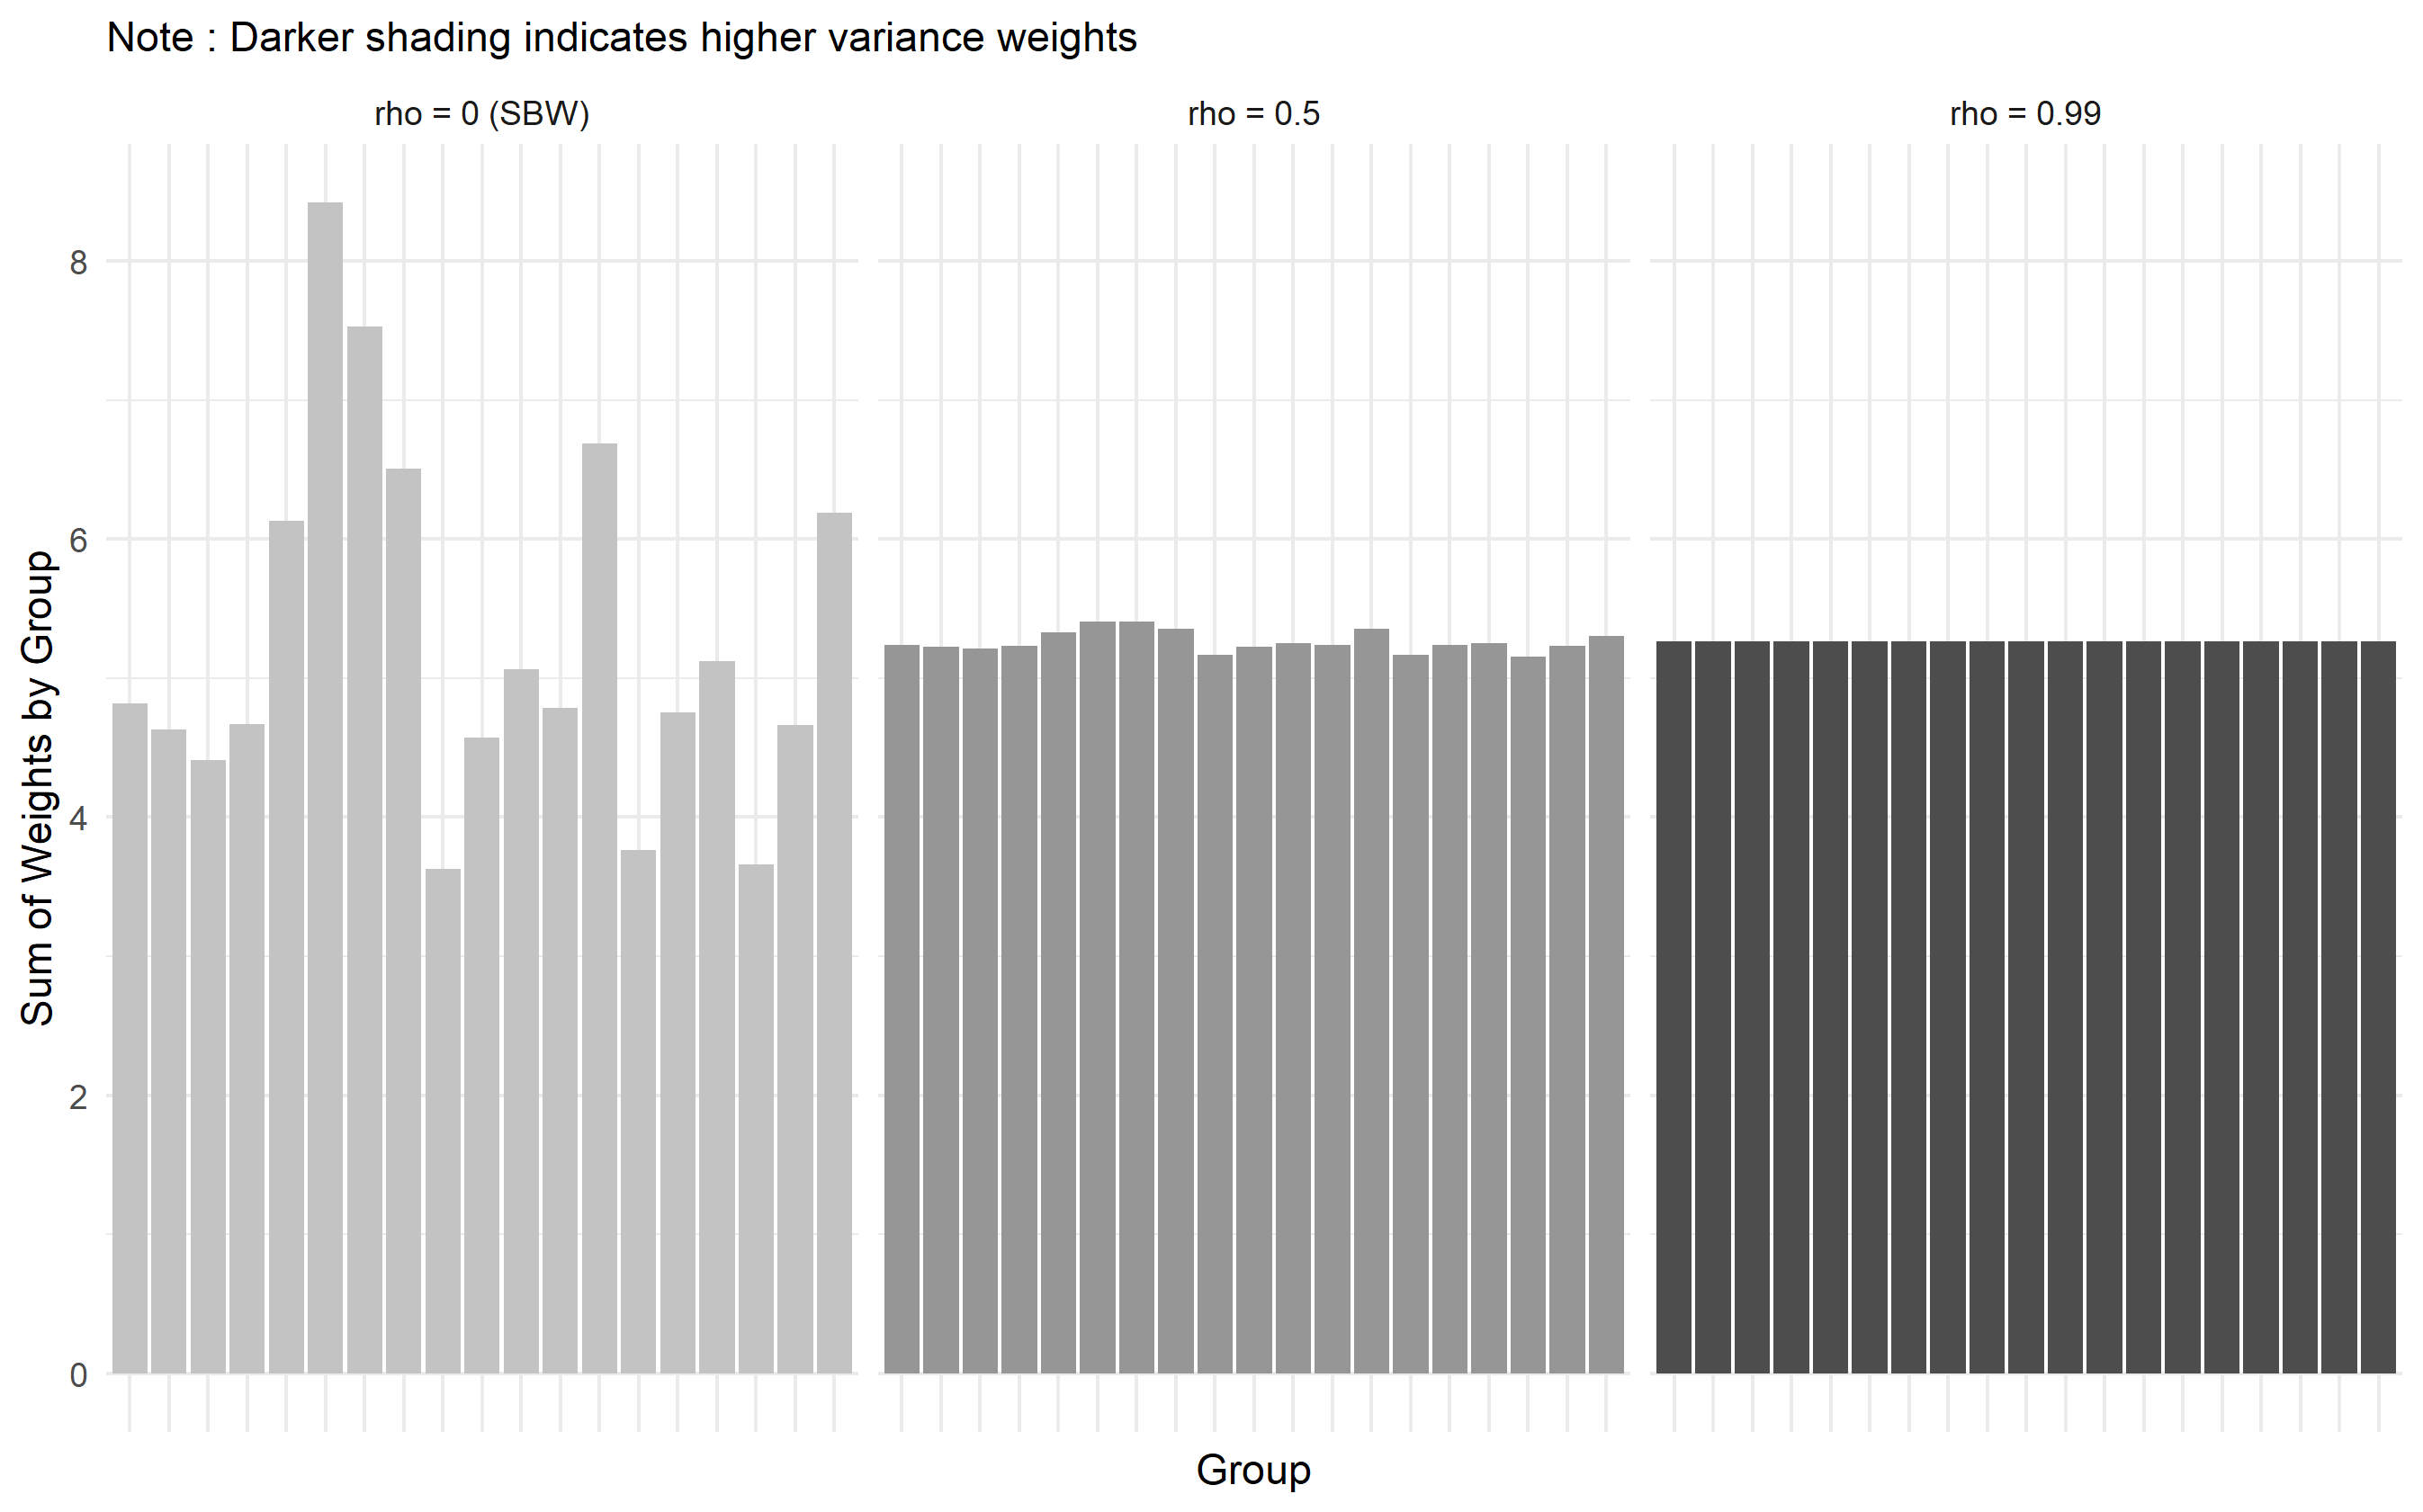
\includegraphics[scale=0.5]{01_Plots/proofofconcept.png}
    \caption{Comparison of SBW and H-SBW: within group sum of weights}
    \label{oatepref}
\end{center}
\end{figure}

In Appendix A we show that the H-SBW objective produces the minimum variance estimator under the constraint set for this correlation structure. In theory we could incorporate any assumed correlation structure into this objective in a similar fashion; however, the number of tuning parameters might change. Broadly speaking, we can think of H-SBW being to SBW what generalized least squares (GLS) is to ordinary least squares (OLS): both SBW and OLS can produce unbiased estimates of model parameters, but H-SBW and GLS can improve the efficiency of an estimator under different assumptions about the correlation structure of the outcomes.

\subsubsection{Measurement error}\label{ssec:methodsmsrment}

A second advancement in our estimation procedure comes in our balance constraints: rather than reweighting the observed covariates, we instead reweight the adjusted estimates $\hat{\eta}_1(W_{sc})$. This helps correct for the estimation error in the covariates that may bias the SBW estimate of $\bar{Y}_0^1$. In Appendix A, we consider the super-population target $\psi^1_0 = \mathbb{E}\{Y^1 \mid A = 0\}$ and show that under the classical errors-in-variables model, the bias for the SBW estimator that balances on the observed covariates $W$ and sets $\delta = 0$ is equivalent to the bias of a linear combination of coefficient estimates from the OLS-based regression estimator. Specifically, the bias for either estimator is:

\begin{equation}
\mathbb{E}\{\hat{\psi}^{1}_0 - \psi^1_0\} = (\upsilon_0 - \upsilon_1)^T(\kappa_1 - I_d)\beta_1
\end{equation}

The intuition for this result is as follows: exact balancing weights implicitly estimate $\beta_1$ on a subset of the data where we have sufficient covariate overlap. We can thus think of SBW as returning a solution to some weighted-least squares problem. Assuming that the outcome model holds across all of the data, WLS and OLS are estimating the same $\beta_1$; consequently, the bias that effects the least squares solution will have the same effect on the WLS, and therefore SBW, solution. In Appendix A, Proposition 2, we show that if we had access to $\eta_1$, we can obtain an unbiased estimate of $\psi^1$ by reweighting the adjusted covariates $\eta_1(W_{sc})$. Of course, in practice we do not know $\eta_1$ but must instead estimate it using auxillary data. In Appendix A, Proposition 3, we show that we can obtain a consistent of $\psi^1$ when balancing on an estimate of $\eta_1$ using auxillary data. 

The key is estimating $\eta_1$: at a high-level, we use the ACS micro-data replicate survey weights to estimate the covariance matrix of CPUMA sampling-variability $\Sigma_{vv, sc}$. Using our observed data to estimate $\Sigma_{WW \mid A = 1}$ and $\bar{X}_1$, we combine these estimates to generate an estimate of $\eta_1$. This is a technique that comes from the regression-calibration literature (see, e.g., \cite{gleser1992importance}). We also consider an adjustment procedure that further accounts for the differential measurement error due to the highly variable sample sizes used to calculate each covariate. This procedure allows our adjustment to differentially adjust covariate values depending on the sample-sizes involved in the adjustment procedure. We refer to the first procedure as ``homogeneous adjustment'' and the second procedure as ``heterogeneous adjustment'' since the adjustment is constant for all units in the first case, but varies by unit in the second case. Further details about these procedures are available in Appendix B. 

This is the first application we are aware of to apply regression calibration in the context of balancing weights to address the problem of measurement error. We emphasize two critical assumptions for using this procedure in our context: (1) the outcome model is linear in the true covariates; and (2) the measurement error in the outcome is uncorrelated with the measurement error in the covariates. The first assumption is strong, though often used in practice. The second assumption is reasonable in our setting, because the outcomes are estimated from a different cross-section than the covariates. 

\subsubsection{Bias-correction for imbalances}

In practice we are unable to reduce the balance constraints to our preferred level without generating very extreme weights. Following the recent literature on synthetic controls, we test the sensitivity of our results to the imbalances in the observed (or adjusted) covariates using ridge-regression augmented weights \cite{ben2018augmented}. Letting $\hat{X}_1$ be the matrix of adjusted covariates, and $\gamma^{hsbw}$ be our H-SBW weights, we consider the regression-augmented weights:

\begin{equation}
\gamma^{aug} = \gamma^{hsbw} + (\gamma^{hsbw}\hat{X}_1 - \bar{W}_0)^T(\hat{X}_1^T\Omega^{-1}\hat{X}_1 + \lambda I_q)^{-1}\hat{X}_1^T\Omega^{-1}
\end{equation}

where $\Omega$ is a block diagonal matrix with diagonal entries equal to one and the within-group off diagonals equal to $\rho$. We choose $\lambda$ so that all imbalances fall within 0.5 percentage points. The cost of this procedure is that we must extrapolate beyond the support of the data, making our estimates more model dependent. We refer to \cite{ben2018augmented} for more details about this procedure. For our results we consider estimators using SBW ($\rho = 0$), H-SBW ($\rho = 1/6$), and ridge-augmented versions of SBW and H-SBW that we call BC-SBW and BC-HSBW. 

\subsection{Model validation}

We previously argued that using pre-treatment outcomes to learn about variable importance may be misleading in this setting. The challenge again is that it is not obvious why the best model of $\bar{Y}_{0, t}^0$ for $t < T$ should also be the best model, or even a good model, of $\bar{Y}^1_{0,T}$. However, for fixed covariates and targeted levels of imbalance $\delta$, we use the heuristic that a good model of $\bar{Y}^1_{0,T}$ should also be a good model of $\bar{Y}_{0, t}^0$. We can also assume that when comparing two models, one with uniformly better covariate balance than the other, the model with uniformly better covariate balance should have lower bias both for $\bar{Y}_{0, T}^1$ and $\bar{Y}_{0, t}^0$ if our model assumptions are correct. We justify these comparisons by again assuming the outcome model is linear in $X$ for all time periods $t$. This is a stronger assumption than necessary to estimate the ETC, which only requires that $\mu_{1, T}$ is linear in $X$. However, these assumptions allow us to at least heuristically compare our models. 

Specifically, we rerun our procedures on pre-treatment data to compare the performance of our models for a fixed level of imbalances $\delta$. In particular, we train our model on 2009-2011 data to predict 2012 outcomes, and 2010-2012 data to predict 2013 outcomes. We limit to one-year prediction error since our estimand is only one-year forward. We then examine the performance of H-SBW against SBW, which vary with respect to the tuning parameter $\rho$, the bias-corrected versions, and the covariate adjustment procedure used in the balancing constraints. 

We expect that the estimators trained on the adjusted data should perform better than the estimators trained on the unadjusted data. If our outcome model is correct, these estimators should achieve better balance across the true covariates and therefore have lower bias than the estimators trained on the unadjusted data. We assume that any difference between the performance of the two adjustments is due to improved balance on the (unobserved) true covariates. For this comparison we do use the performance on this data to choose which adjustment we prefer for our final results. Conditional on the adjustment, we assume that if the bias-corrected estimators all have uniformly better covariate balance than the uncorrected estimators, these estimators should also perform better than the uncorrected estimators. However, if the assumed outcome models are incorrect, these estimators may suffer from extrapolation bias and perform worse despite achieving better balance. Finally, we expect SBW to have similar performance to H-SBW. We do expect to find the variance of H-SBW to be lower; however, we are only able to observe predictions on two years of pre-treatment data.

\subsection{Inference}

While placebo tests are frequently used in the synthetic controls literature for inference, we view these as qualitative statistical tests (see, e.g., \cite{arkhangelsky2019synthetic}) and instead use the leave-one-state-out jackknife to estimate the variance of $\hat{Y}_0^1$ (\cite{cameron2015practitioner}). Specifically, we exclude each state and re-calculate the weights holding our targeted mean fixed at $\bar{X}_0$ (using our estimate $\bar{W}_0$ and ignoring the variability associated with these estimates).\footnote{When our preferred initial choice of $\delta$ does not converge, we gradually reduce the constraints until it does.} We compute this estimate in two ways: first, we condition on our covariate adjustment $\hat{\eta}_1$. This is our preferred estimator; however, it does not account for the randomness in $\hat{\eta}_1$. We conduct a second procedure where we re-estimate $\hat{\eta}_1$ for each state omitted in the jackknife procedure and provide these results in Appendix E.

To estimate the variance of $\bar{Y}_0^0$ we use an auxillary regression model and use the CR-2 standard error adjustment to estimate the variance of the linear combination $\bar{W}_0^T\hat{\beta}_0$. We can estimate this quantity using the original (unadjusted) data given that $\mathbb{E}_W\{\bar{W}_0^T\hat{\beta}_0\} = \bar{Y}_0^0$ (since the regression line runs through the point $(\bar{W}_0, \bar{J}_0)$, which are unbiased estimates of $(\bar{X}_0, \bar{Y}_0)$). Our final estimate is the sum of these two variance estimates, and we use standard normal quantiles to generate confidence intervals. 

\section{Results}

We first present summary statistics regarding the variability of six time-varying covariates on our adjusted and unadjusted datasets. The second sub-section contains covariate balance diagnostics. The final sub-section contains our ETC estimates.

\subsection{Covariate adjustment}

Table~\ref{tab:adjust1} displays the effects of our covariate adjustment procedure on the variance of our pre-treatment outcomes and pre-treatment unemployment rates among the expansion states. We most heavily prioritize balancing these covariates, but they are also among the least precisely estimated (all of our other covariates average over multiple years of data). Table~\ref{tab:adjust1} displays the variance of each covariate on the unadjusted and adjusted datasets. We see that both the homogeneous and heterogeneous adjustment procedures reduce the variability in the data by comparable amounts. Intuitively, these adjustment reduce the likelihood that our balancing weights will over-fit to noise in the data. These results are consistent across most of our other covariates.

\begin{table}[ht]
\caption{Sample variance on unadjusted and adjusted datasets, expansion states}
\label{tab:adjust1}
\begin{tabular}{lrrr}
  \hline
Variable & No adjustment & Heterogeneous & Homogeneous \\ 
  \hline
Uninsured Pct 2011 & 8.35 & 8.04 & 8.05 \\ 
  Uninsured Pct 2012 & 8.20 & 7.89 & 7.90 \\ 
  Uninsured Pct 2013 & 8.09 & 7.78 & 7.79 \\ 
  Unemployed Pct 2011 & 3.66 & 3.25 & 3.27 \\ 
  Unemployed Pct 2012 & 3.72 & 3.38 & 3.38 \\ 
  Unemployed Pct 2013 & 3.20 & 2.88 & 2.87 \\ 
   \hline
\end{tabular}
\end{table}

\subsection{Covariate balance}

Figure~\ref{fig:loveplotc1} displays the reduction of imbalances using our H-SBW weights. This plot only displays covariates with greater than one percentage point difference between the targeted mean in the expansion region and the mean values in the non-expansion region prior to weighting, and the reweighted treatment values use our preferred covariate adjustment $\hat{\eta}_1(W_{sc})$. Before applying our weights, we see that there are substantial imbalances in the Republican governance indicators, as well as pre-treatment uninsurance and unemployment rates. Our weights reduce these differences; however, some remain, particularly among the Republican governance indicators. A complete balance table is available in Appendix D, Table 4. 

\begin{figure}[H]
\begin{center}
    \caption{Balance plot, primary dataset}
    \label{fig:loveplotc1}
    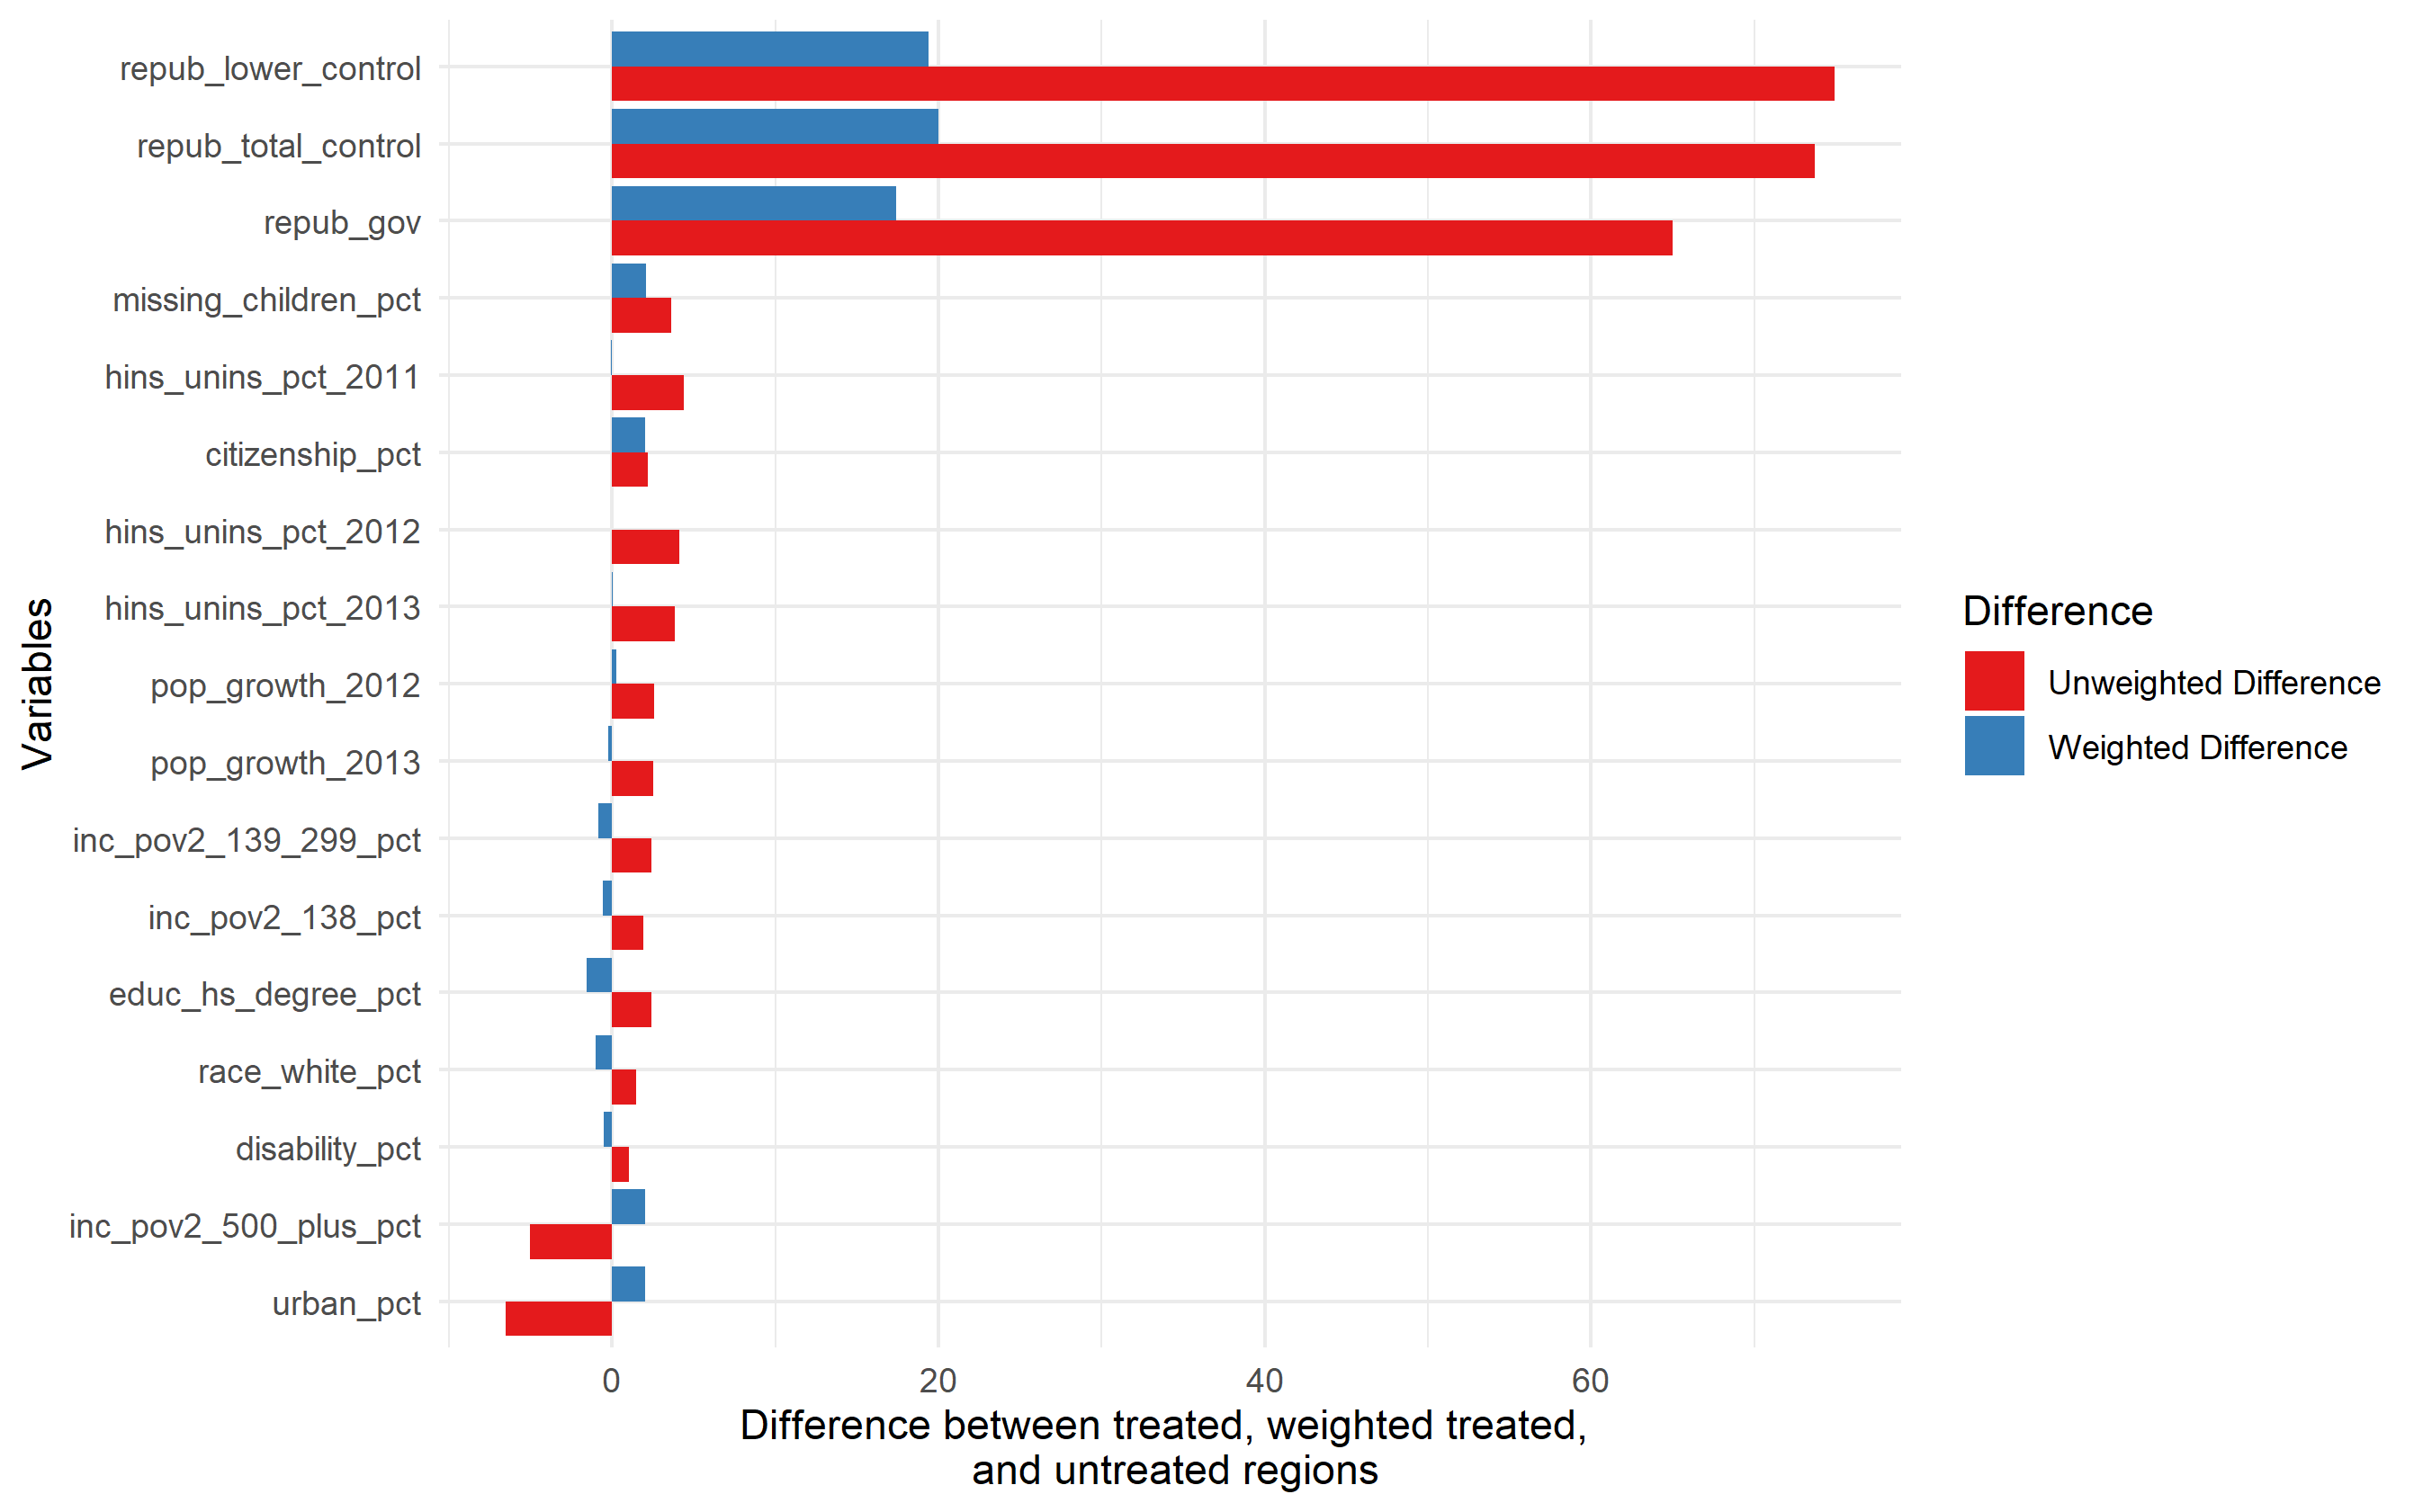
\includegraphics[scale=0.5]{01_Plots/balance-plot-etuc1.png}
\end{center}
\end{figure}

\begin{figure}[H]
\begin{center}
    \caption{H-SBW versus BC-HSBW versus SBW, weights summed by state, primary dataset}
    \label{fig:sbwvhsbw1}
    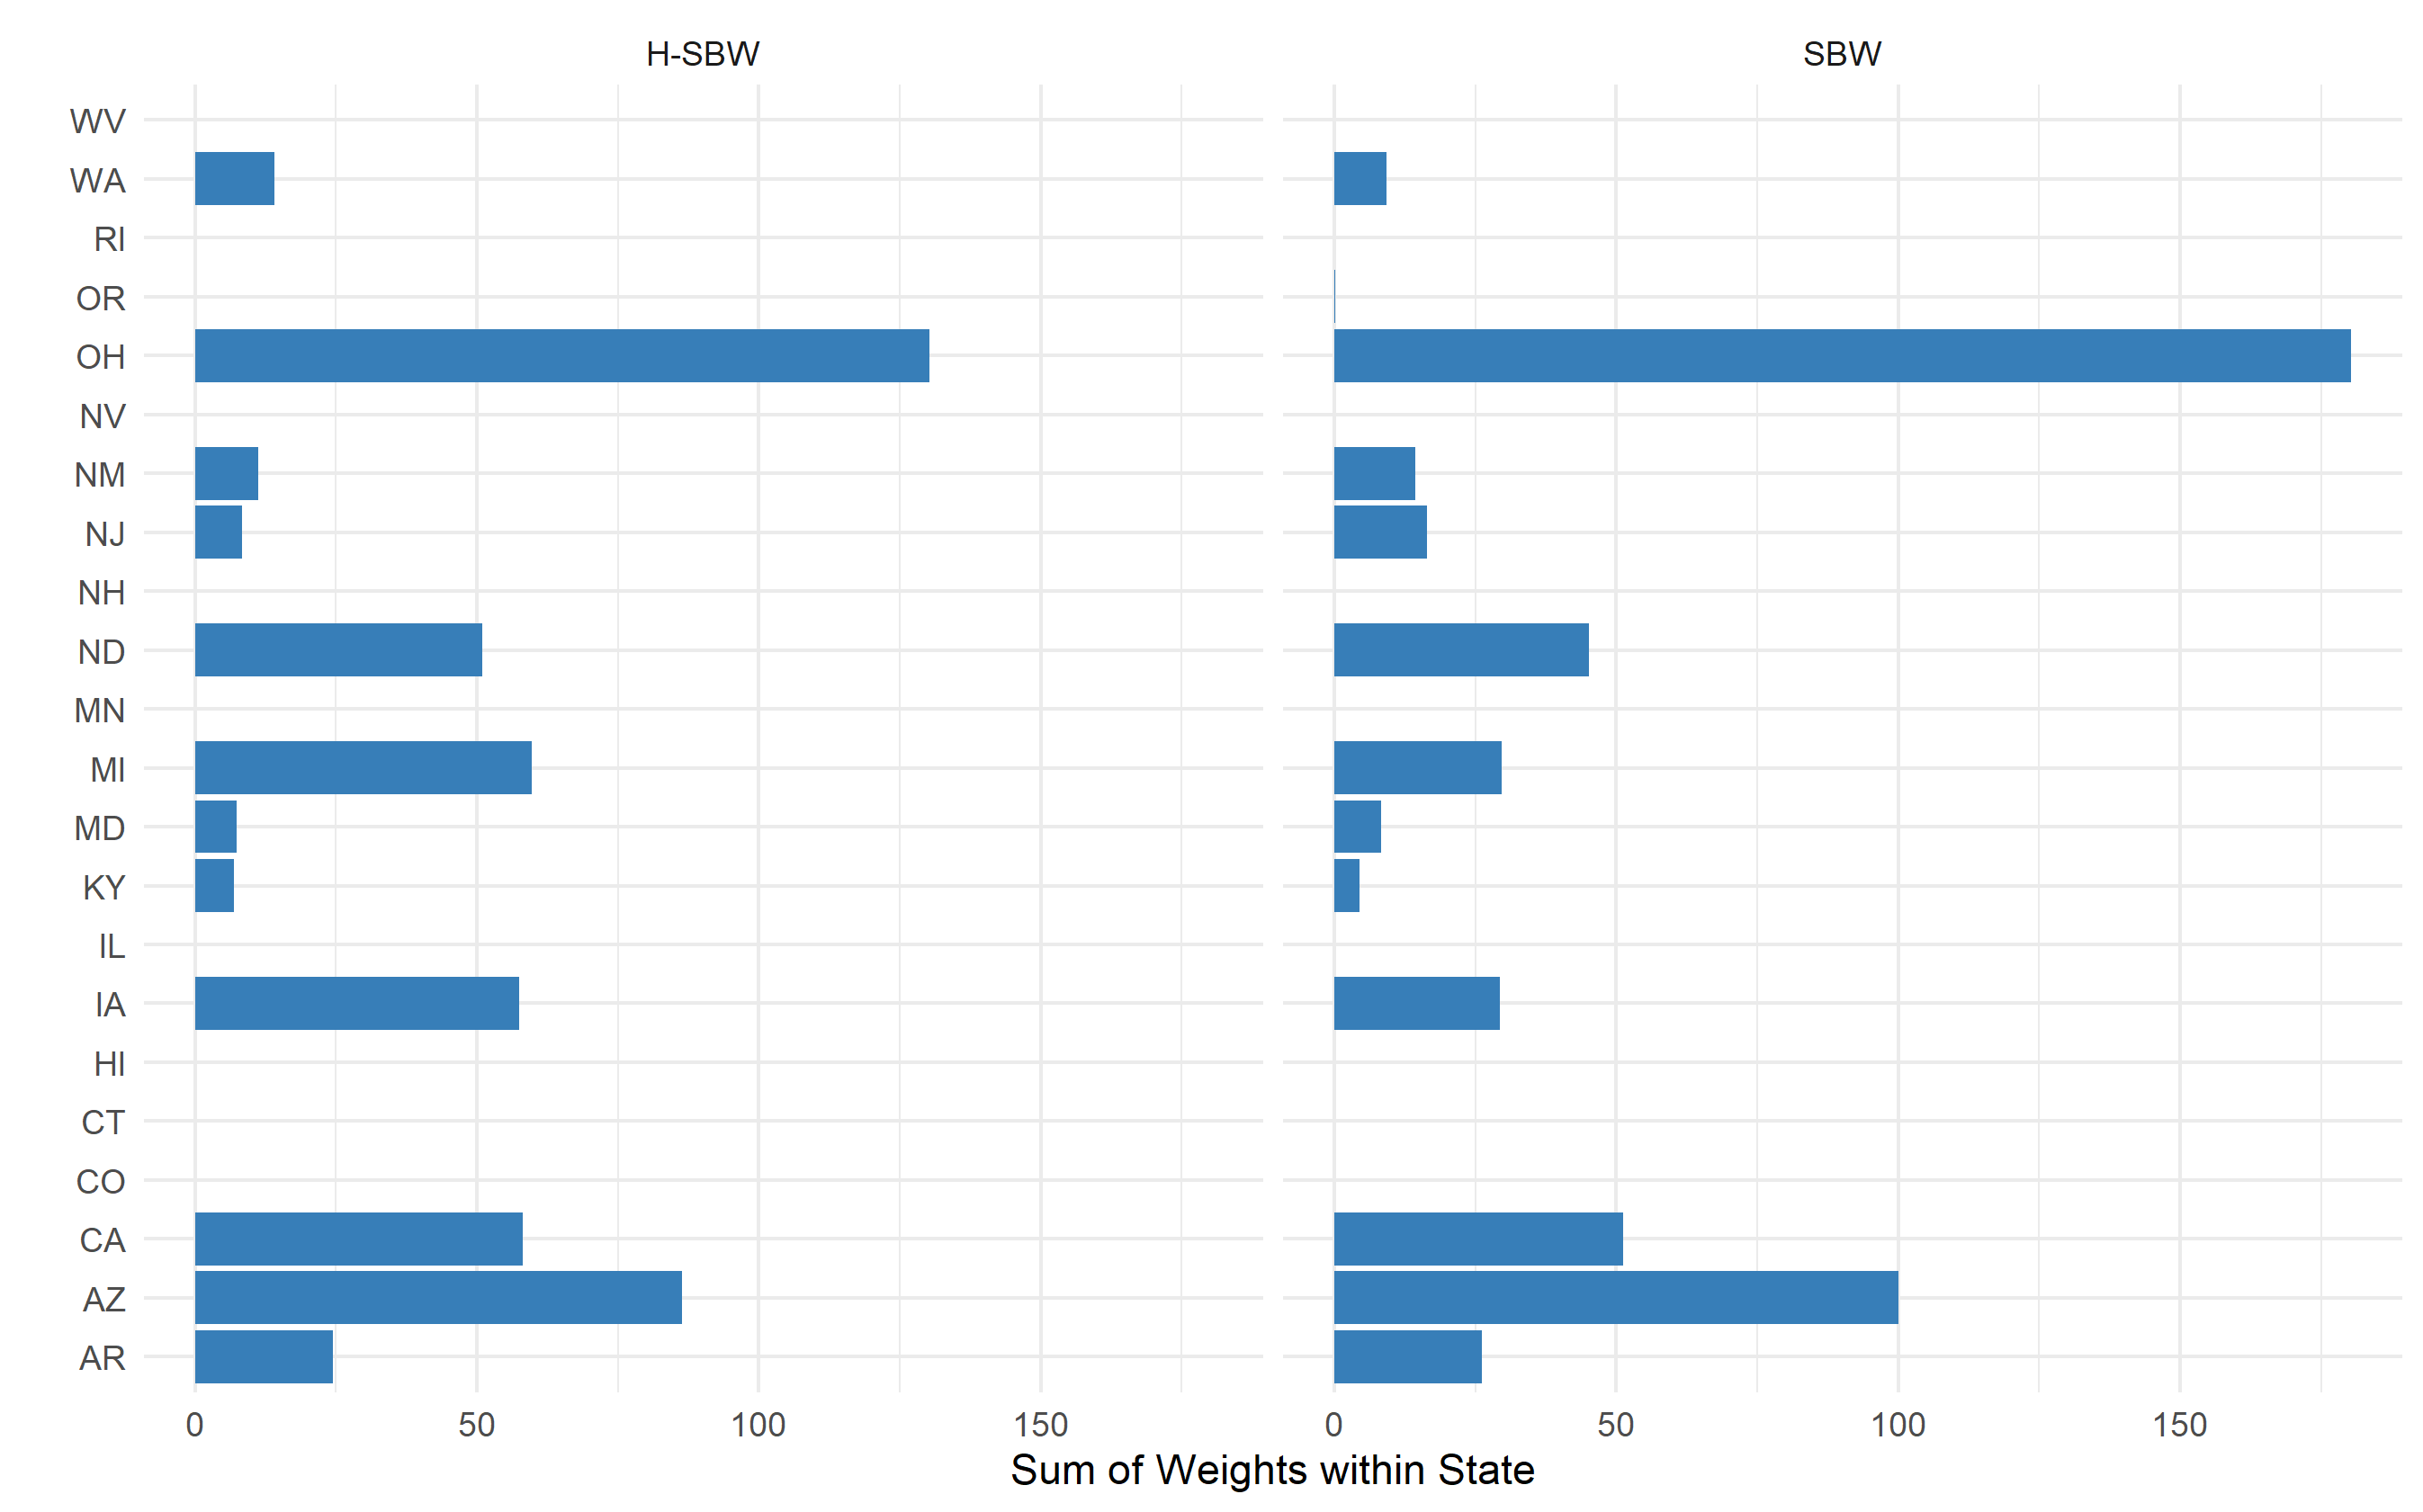
\includegraphics[scale=0.6]{01_Plots/weights-by-state-sbw-hsbw-c1.png}
\end{center}
\end{figure}

We then use ridge-regression augmentation to extrapolate from the data in order to reduce all imbalances within 0.5 percentage points. Figure~\ref{fig:sbwvhsbw1} shows the total weights summed across states for three estimators: H-SBW, BC-HSBW, and SBW. For BC-HSBW we display the negative weights separately from the positive weights to show the extent of the extrapolation. This figure illustrates two key points: first, that H-SBW more evenly disperses the weights across states relative to SBW; second, that BC-HSBW extrapolates somewhat heavily in order to achieve the desired level of balance, particularly for CPUMAs in California. 

Finally, we examine whether the H-SBW weights generated using the unadjusted data balance the adjusted covariates. While this metric does not reflect the ``true'' imbalances, the comparison gives some indication of whether the unadjusted weights are overfitting to noisy covariate measurements. [add sentence on what to expect] Table~\ref{tab:balcomp} compares the imbalances among our pre-treatment outcomes and uninsurance rates using H-SBW weights generated on our unadjusted dataset applied to the adjusted (homogeneous) dataset. The ``Unweighted Difference'' column represents the raw difference in means, while the ``Weighted Diff'' column reflects the weighted difference that we calculate on the unadjusted dataset. The ``Homogeneous Diff'' column displays the weighted imbalance when applying the H-SBW weights to the dataset using the homogeneous adjustment, and likewise for ``Heterogeneous Diff.'' The weighted pre-treatment outcomes are approximately one percentage point lower than we desired in the two years prior to treatment using the heterogeneous adjustment, and -0.2 percentage points lower (on average) using the homogeneous adjustment. Compared with the weighted difference (no adjustment) this is suggestive that the unadjusted weights are overfitting to noisy covariates and may give an overly optimistic view of balance obtained. Given the high degree of expected correlation between pre-treatment and post-treatment outcomes, we may expect the estimator of $\bar{Y}^1_0$ trained on the unadjusted data to have a downward bias.

\begin{table}[ht]
\caption{Balance comparison: weights estimated on unadjusted data applied to adjusted data}
\label{tab:balcomp}
\begin{tabular}{lrrrr}
  \hline
Variables & Unweighted Diff & Weighted Diff (none) & Homogeneous Diff & Heterogeneous Diff\\ 
  \hline
Uninsured Pct 2011 & -3.09 & -0.05 & -0.11 & 0.92 \\ 
  Uninsured Pct 2012 & -2.99 & -0.05 & -0.21 & -1.06 \\ 
  Uninsured Pct 2013 & -3.00 & -0.05 & -0.38 & -0.93 \\
   \hline
\end{tabular}
\end{table}

\subsubsection{Model validation}

We compare the performance of our models by repeating the covariate adjustments and calculating our procedure on 2009-2011 ACS data to predict 2012 outcomes, and similarly for 2010-2012 data to predict 2013 outcomes for the treated states. From Table~\ref{tab:pretxpred} we see that the estimators trained on the covariate adjusted data have substantially better performance than the unadjusted data. Moreover, the estimators trained on the homogeneous adjustment seem to do slightly better than the ones that model the heterogeneity; we present our results using the homogeneous adjustment. In thees earlier years we find that SBW tends to have slightly lower RMSE than H-SBW. However, the results are quite similar, as we expected. Finally, we see that the bias corrected estimators tend to perform worse in this application. This may indicate that the extrapolation bias outweighs the cost of reducing the covariate imbalances. While this does not imply that this model will perform badly when predicting $\bar{Y}^1_T$, it does suggest caution regarding these results. We see this as a function of our models being approximations: we expect in general that assuming the linear outcome models approximately holds on the support of the data where we have sufficient covariate overlap; however, these models may lead us astray when our weights extrapolate excessively from the data. The worst performing estimators are the bias-corrected estimators trained on the unadjusted data.

\begin{table}[ht]
\caption{Estimator pre-treatment outcome prediction error}
\label{tab:pretxpred}
\begin{tabular}{llrrr}
  \hline
Sigma estimate & Estimator & 2012 error & 2013 error & RMSE \\ 
  \hline
Homogeneous & SBW & -0.18 & -0.22 & 0.20 \\ 
  Homogeneous & H-SBW & -0.24 & -0.21 & 0.23 \\ 
  Heterogeneous & SBW & -0.25 & -0.30 & 0.27 \\ 
  Heterogeneous & H-SBW & -0.32 & -0.39 & 0.36 \\ 
  Homogeneous & BC-SBW & -0.42 & -0.35 & 0.39 \\ 
  Heterogeneous & BC-SBW & -0.45 & -0.39 & 0.42 \\ 
  None & SBW & -0.50 & -0.61 & 0.56 \\ 
  None & H-SBW & -0.52 & -0.61 & 0.57 \\ 
  Homogeneous & BC-HSBW & -0.53 & -0.62 & 0.58 \\ 
  Heterogeneous & BC-HSBW & -0.53 & -0.72 & 0.63 \\ 
  None & BC-SBW & -0.82 & -0.93 & 0.88 \\ 
  None & BC-HSBW & -0.93 & -0.99 & 0.96 \\ 
   \hline
\end{tabular}
\end{table}

We find a consistent negative bias across all of our estimators: all of our models tend to under-predict the true uninsurance rate among the non-expansion states the subsequent year by between a fifth to a whole percentage point. Assuming that the sign of this bias will also affect our estimates of $\bar{Y}^1_0$, we should expect our treatment effect estimates to have slight downward bias. That is, the true treatment effect may be smaller (closer to zero) in absolute magnitude than the estimated treatment effect. 

\subsection{Primary Results}

Using H-SBW we estimate an effect of -2.33 (-3.49, -1.16) percentage points. The SBW results are almost identical with -2.35 (-3.65, -1.06) percentage points. Compared to the unadjusted data we see very similar estimates at -2.34 (-2.85, -1.82) percentage points for H-SBW and -2.39 (-2.95, -1.83) percentage points for SBW. We see that H-SBW reduces the confidence intervals relative to SBW. We also observe that using the adjusted covariate set increases the width of the estimated confidence intervals. This increase in variability is expected because the adjustment procedure generally reduces the variability in the data, as we saw in Table~\ref{tab:adjust1}, thereby requiring that the balancing weights also increase in variability to achieve the desired level of balance. Importantly, this variance estimate conditions on the covariate adjustment, and does not take into account the randomness in this procedure, and may understate the true uncertainty. When we recalculate the entire adjustment procedure, we find that the confidence intervals are of a comparable magnitude. The results are available in Appendix E.

When we add the bias-correction, the absolute magnitude of the point estimate decreases: we estimate -2.05 (-3.32, -0.79) percentage points for BC-HSBW and -2.00 (-2.98, -1.01) percentage points for BC-SBW. Interestingly, in contrast to our validation tests, where the bias-corrected estimators tended to predict lower uninsurance rates than the other estimators, here the bias-correction predicts higher uninsurance rates for $\bar{Y}^1_0$. We also see that in contrast to the H-SBW and SBW estimators, the confidence interval for BC-SBW is narrower than for BC-HSBW. Table~\ref{tab:mainresults} presents all of our estimates, along with the results when excluding early expansion states. All adjusted estimates were closer to zero than the unadjusted estimates, though the point estimates from the SBW and H-SBW were estimators were virtually identical. We briefly note that the heterogeneous adjustments were all closer to zero than the unadjusted estimates. Complete results are available in Appendix E.

\begin{table}[ht]
\label{tab:mainresults}
\caption{Primary results}
\begin{tabular}{llll}
  \hline
Weight type & Adjustment & Estimate (95\% CI) & Early excluded estimate (95\% CI) \\ 
  \hline
H-SBW & Homogeneous & -2.33 (-3.49, -1.16) & -2.09 (-2.85, -1.33) \\ 
  H-SBW & None & -2.34 (-2.85, -1.82) & -2.28 (-2.82, -1.74) \\ 
  BC-HSBW & Homogeneous & -2.05 (-3.27, -0.82) & -1.94 (-2.96, -0.92) \\ 
  BC-HSBW & None & -2.22 (-2.87, -1.56) & -2.22 (-3.07, -1.38) \\ 
  SBW & Homogeneous & -2.35 (-3.65, -1.06) & -2.05 (-2.75, -1.35) \\ 
  SBW & None & -2.39 (-2.95, -1.83) & -2.21 (-2.71, -1.72) \\ 
  BC-SBW & Homogeneous & -2.07 (-3.17, -0.97) & -1.99 (-3.00, -0.99) \\ 
  BC-SBW & None & -2.19 (-2.90, -1.49) & -2.23 (-3.05, -1.40) \\ 
   \hline
\end{tabular}
\end{table}

We also consider the sensitivity of our analysis with respect to no anticipatory treatment effects. We exclude California, Connecticut, Minnesota, New Jersey, and Washington, which had partial expansions prior to 2014, and rerun our analyses. Figure 2 in Appendix D displays the H-SBW weights summed by state alongside BC-HSBW, which extrapolates to reduce the imbalances, and the results are available in Table~\ref{tab:mainresults}.

Our point estimates are similar to our primary analysis, though the numbers move slightly closer to zero. We also see that the differential between the estimates on the adjusted and unadjusted data is slightly larger: -2.28 (-2.82, -1.74) percentage points for H-SBW on the unadjusted dataset and -2.09 (-2.85, -1.33) on the adjusted data. We again find that when we add the bias-correction the point estimates again move closer to zero. Overall our primary results are relatively robust to the exclusion of these states. We conclude that potential violations of this causal assumption are not a large factor.

Lastly, we examine the robustness of our point estimates to the removal of individual states (these are the same point estimates used to calculate our confidence intervals). We find that removing Ohio tends to move the point estimates farther from zero, while removing North Dakota, Kentucky, or California tends to move the estimates closer to zero. Appendix E Figure 3 displays a heatmap showing how the estimates change for each estimator when removing each state.

\section{Discussion}

We estimate that had states that did not expand Medicaid in 2014 instead expanded their programs, they would have seen a -2.33 (-3.49, -1.16) percentage point change in the adult uninsurance rate. Existing estimates place the ETT between -3 and -6 percentage points. These estimates vary depending on the targeted sub-population of interest, the data used, the level of modeling (individuals or regions), and the modeling approach (see, e.g., \cite{courtemanche2017early}, \cite{kaestner2017effects}, \cite{frean2017premium}). Our estimate of the ETC are closer to zero than these ETT estimates. This difference may be a function of these different modeling strategies, or it may suggest that the ETC is smaller in absolute magnitude than the ETC. Regardless, due to the potential for effect heterogeneity, we emphasize the importance of directly estimating the targeted counterfactual of interest (e.g. the ETT or ETC), and being explicit about the assumptions used to estimate these quantities. We now consider our methodological contributions, study limitations, and we conclude by considering the policy implications of these findings.

\subsection{Methodological considerations}

We provide several methodological contributions to the literature on synthetic controls and balancing weights. First, we clarify some of the assumptions required to use synthetic controls to estimate the ETC. The challenge is that we need to predict treatment response rather than the outcome absent treatment. We emphasize that there may exist covariates that are weak confounders of the outcome absent treatment, but are strong confounders of the outcome under treatment.\footnote{In Appendix F we consider the role of Republican governance as an example, noting that \cite{kaestner2017effects} and \cite{courtemanche2017early} do not control for these factors when estimating their synthetic control weights. We show that these factors do substantially influence our estimates of $\bar{Y}_0^1$, though this does not rule out that these factors may also matter for predicting $\bar{Y}_1^0$.} While perhaps obvious, this point is not fully appreciated in the applied literature. For example, \cite{born2020lockdowns} recently used synthetic controls to estimate Sweden's COVID cases and deaths had they instituted a lockdown. The authors balance on pre-treatment infections, urbanization rate, and population size, and argue that the treatment is effectively random conditional on these covariates. While this may be true, the authors use the standard synthetic controls algorithm to generate their weights, using pre-treatment outcomes to determine the best model of the post-treatment counterfactual of $\bar{Y}^1_0$. For this application we forego this type of procedure and instead use our prior knowledge about the problem to prioritize covariate balance.

Second, our estimation procedure introduces and illustrates the H-SBW objective, which can improve upon the SBW objective when using hierarchical data. Assuming the errors in the outcome model follow the covariance structure posited by \cite{kloek1981ols}, H-SBW produces a lower variance estimator by more evenly dispersing weights across states. The assumption underlying the particular structure of our objective is that our model errors have constant variance and constant within-state correlation $\rho$. However, our procedure requires assuming the covariance structure and $\rho$ in advance. We choose $\rho = 1/6$ for this application. Identifying a data-driven approach to choose this tuning parameter (or perhaps for the covariance structure in general) could be a useful future contribution. 

Third, our estimation procedure accounts for measurement error in our covariates. We modify the constraint set to balance on a linear approximation to the true covariate values by adapting regression-calibration techniques (\cite{gleser1992importance}) to the balancing weights context. In Table~\ref{tab:balcomp} we show that the weights calculated on the unadjusted dataset fail to achieve the desired level of covariate balance on the adjusted dataset. We find that the weighted imbalances in our pre-treatment outcomes may be larger than we wanted, which we speculate for this application might bias our treatment effect downward. When we compared our estimates using the adjusted covariates to the unadjusted covariates, we find that our point estimates decrease (although often only slightly) in absolute magnitude. Essentially, when we generate weights on the unadjusted data to estimate the 2014 counterfactual outcome, they are likely fitting to noise, causing the observed level of balance to appear better than it truly is. Meanwhile, the re-weighted region may suffer from regression to the mean in the post-treatment period, making our treatment effect estimates appear larger in absolute magnitude than the truth. Once we adjust for the measurement error, our point estimates decrease in absolute magnitude (see also \cite{daw2018matching}, who discuss this phenomenon in more detail in the context of difference-in-differences designs). Overall, our study provides a roadmap for future studies that may wish to correct for potential measurement error while using balancing weights. 

One direction for further work is to calibrate this procedure to determine an optimal bias-variance tradeoff with respect to the measurement error. The procedure we implemented here was likely sub-optimal with respect to the mean-square error of our estimator. In particular, the bias induced by the measurement error decreases with square root of the sample size used to calculate each CPUMA's covariate values, the minimum of which were over three hundred. Meanwhile, the variance of our counterfactual estimate should decrease with the square root of the number of treated states (of which there are 21). From a theoretical perspective, the variance is of a larger order than the bias; moreover, adjusting for the bias will further increase the variance of the estimator. These concerns are consistent with our observed results: the change in our point estimates from the unadjusted data to the adjusted data is of a smaller magnitude than our variance estimate on our point estimate on the unadjusted data. Moreover, once we adjust for the measurement error, our confidence intervals increase more widely than the point estimates change.

\subsection{Limitations}

We caution that we required strong modeling assumptions throughout this analysis. In particular, we require SUTVA, no anticipatory treatment effects, no unmeasured confounding conditional on the true covariates, and several parametric assumptions about both the outcome and measurement error models. We were able to address some concerns about possible violations of these assumptions. For example, our results were qualitatively similar whether we excluded possible ``early expansion states,'' or used different weighting strategies (including relaxing the positivity restrictions and changing the tuning parameter $\rho$). We also examined two versions of our covariate adjustment and found similar results with either. However, we do not attempt to address concerns about SUTVA violations, particularly the impact of spillovers across regions. And while we believe that no unmeasured confounding is reasonable for this problem, we did not conduct a sensitivity analysis (see, e.g., \cite{bonvini2021sensitivity}) with respect to this assumption.

\subsection{Policy considerations}

We find that our point estimates for the ETC are somewhat smaller in absolute magnitude than existing estimates of the ETT. While we make no formal statistical claims about these differences, this finding nevertheless highlights the importance of caution when using estimates of the ETT to make inferences about the ETC. Because almost every outcome of interest is mediated through increasing the number of insured individuals, if the ETC is in fact different than the ETT, then projecting findings from an estimate of the ETT to the ETC may lead to inaccurate inference. For example, \cite{miller2019medicaid} study the effect of Medicaid expansion on mortality. Using their estimate of the ETT they project that had all states expanded Medicaid, 15,600 deaths would have been avoided during their study's time-period. If we believe that this number increases monotonically with the number of uninsured individuals, this estimate may be an overestimate if the ETC is less than the ETT, or an underestimate if the ETC is greater than the ETT. Directly estimating the ETC can help us better model policy relevant downstream effects mediated through decreasing the uninsurance rate. 

Medicaid expansion is also still an ongoing policy debate in the United States. Following the passage of the American Rescue Plan, state legislatures in Wyoming, Alabama, and North Carolina are reportedly considering expanding their programs. Our study estimates the effect of Medicaid expansion on adult uninsurance rates; however, this effect is only interesting because Medicaid enrollment is not automatic for eligible individuals. Different state policies may therefore make it easier or harder to enroll in Medicaid. We emphasize that if the goal of Medicaid expansion is to increase insurance access for low-income adults, state policy-makers also may wish to make it easier to enroll in Medicaid. 

\section{Conclusion}

This is the first study we are aware of that directly estimates the foregone coverage expansions of Medicaid expansion on states that did not expand Medicaid in 2014. Our estimation approach contributes to the methodological literature on synthetic controls by outlining a set of identifying assumptions to estimate the ETC rather than the ETT, and to the balancing weights literature by using an estimation procedure that account for hierarchical data structure and measurement error in the covariates. We estimate that had states that did not expand their Medicaid eligibility requirements in 2014 done so, they would have seen a -2.33 (-3.49, -1.16) percentage point change in their uninsurance rate. This point estimate is closer to zero than existing estimates of the ETT, which range between -3 and -6 percentage points (\cite{frean2017premium}).\footnote{As we noted above, prior studies differ with respect to the data used, the targeted population of interest, the modeling choices, and unit level of analysis.} From a policy-analysis perspective, we caution against using using existing estimates of the ETT to make inferences about the ETC. From a policy-making standpoint, we note that if the goal of Medicaid expansion is to increase access to insurance for low-income adults, state and federal policy-makers may wish to consider policies that make Medicaid enrollment easier if not automatic.

\section*{Acknowledgements}

The authors gratefully acknowledge invaluable advice and comments from Zachary Branson, Dave Choi, Edward Kennedy, Brian Kovak, Akshaya Jha, Lowell Taylor, and Jose Zubizaretta.

\begin{supplement}
Analysis programs and supporting materials are available online at github.com/mrubinst757/medicaid-expansion. Proofs and additional results are available in the Appendix.
\end{supplement}

\bibliographystyle{imsart-nameyear} % Style BST file
\bibliography{research.bib}       % Bibliography file (usually '*.bib')

\end{document}
